\section{Preliminary Experiments}
\label{sec:experiment}

Figure~\ref{fig:statistic} shows the results of the experiments. The meaning of each column is described as follows. $original$ column means the results of each column below it are obtained on original programs. $\sharp loc$ means the number of program locations; $\sharp func$ means the number of functions in a program; $cpu time (total)$ means cpu total execution time in seconds; $memory (MB)$ means the number of consumed memory cells by model checker; $fixed num$ means the number of available memory cells; the $true$ or $false$ behind $fixed num$ means it is true if the number of  the memory cells which a program consumes does not exceed the $fixed num$, otherwise it is false; $behavioral$ column means the results of each column below it are obtained on the abstracted behavioral type.

All of the experiments are done on a machine with an Inter(R) Core i5-4590  3.30Hz CPU, 6MB cache and 8GB memory, running Debian (kernel version) and CPAchecker (version 1.3.2). The programs used for the experiments are described as follows:
\begin{itemize}
\item linklist.c and linklist2.c create a list,
\item linkstack.c creates a stack.
\item linkqueue.c creates a queue.
\item binarysorttree.c sorts a binarytree
\item database.c creates a database.
\item ihex2fw.c converts ihex files into binary representation for use by Linux kernel.
\item gen-init-cpio.c produces a binary file which performs on a file containing newline separated entries that describe the files to be included in the initramfs archive
\end{itemize}

The results present in the Figure~\ref{fig:statistic} show that the resources required for model checking become smaller if applying model checkers to the abstracted behavior, since the abstracted behavior only consists of allocation and deallocation.

One thing we should notice in Figure~\ref{fig:statistic} is that the result of true or false in fixe num column may be different under the same program, for example, linklist.c has the true under original column but the false under behavioral column, because



\begin{figure}
 \centering
 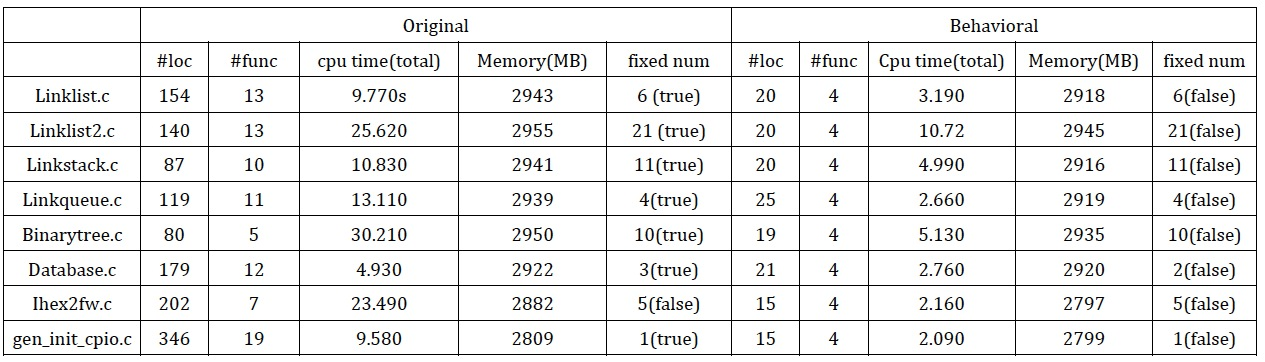
\includegraphics[width=14cm]{statistic.png}
\caption{Comparison}
\label{fig:statistic}
\end{figure}
